
\chapter{Week13}
\section{Wednesday}
\paragraph{Announcement}
This lecture will quickly go through the Morse Lemma, and the constraint optimization problem.

\subsection{Morse Lemma}
Recall that the rank theorem essentially contains the same idea as the SVD decomposition in linear algebra, i.e., we left and right composite functions to the original to obtain its canonical form. Here we study other way of reduction of a smooth real-valued function to its canonical form near a non-degenerate critical point.
\begin{definition}[Non-degenerate critial point]
Let $\bm x_0$ be a critical point of the function $f\in\mathcal{C}^2(U,\mathbb{R}). $
The point $\bm x_0$ is called the \emph{non-degenerate critical point} if the Hessian 
\[
\bm H(\bm x_0)=
\left[
\frac{\partial^2}{\partial x_i\partial x_j}(\bm x_0)
\right]
_{m\times m}
\]
is invertible.
\end{definition}

To show the local performance near the non-degenerate critical point, we apply the Taylor expansion near $\bm x_0$ first:
\begin{equation}\label{Eq:13:1}
\begin{aligned}
f(\bm x)&=f(\bm x_0)+
\frac{1}{2}(\bm x-\bm x_0)\trans\bm H(\bm x_0)(\bm x-\bm x_0)+o(\|\bm x-\bm x_0\|^2)\\
&=f(\bm x_0)+\frac{1}{2}\sum_{i,j=1}^m\frac{\partial^2f}{\partial x_i\partial x_j}(\bm x_0)(x_i-x_{0,i})(x_j-x_{0,j})+o(\|\bm x-\bm x_0\|^2)
\end{aligned}
\end{equation}
where $\bm x = (x_1,\dots,x_m)$ and $\bm x_0=(x_{0,1},\dots,x_{0,m})$. 

The second term in the RHS of (\ref{Eq:13:1}) is a \emph{symmetric quadratic form}. Recall that the linear algebraic approach to deal with the quadratic form $\bm x\trans\bm A\bm x$ is to transform it into $(\bm Q\bm x)\trans\bm\Lambda\bm Q\bm x$ by the eigen-decomposition, the advantage of which is that $\bm\Lambda$ is diagonal and thus this quadratic term is easy to compute. The Morse lemma essentially contains the same idea.

\begin{theorem}[Morse Lemma]
Given a function $f\in\mathcal{C}^3(U(\bm x_0),\mathbb{R})$ such that $U(\bm x_0)\subseteq \mathbb{R}^m$, suppose $\bm x_0\in U$ is a \emph{non-degenerate critical point} of $f$, then there exists a \emph{diffeomorphism} $\phi:V\to U$, where $V\times U$ is some neighborhood $N(\bm 0)\times N(\bm x_0)$ ($\bm0$ denotes the origin for $\mathbb{R}^m$), such that for $\forall \bm y\in V$,
\[
(f\circ \phi)(\bm y)=f(\bm x_0)-(y_1^2+\cdots+y_k^2)+(y_{k+1}^2+\cdots+y_m^2)
\]
\end{theorem}

The proof of Morse Lemma relies on the Hadamard Lemma:

\begin{proposition}[Hadamard Lemma]
Let $f\in\mathcal{C}^p(U,\mathbb{R})$ and $p\ge1$, with $U$ to be a \emph{convex} neighborhood of $\bm0\in\mathbb{R}^m$, and $f(\bm0)=0$. Then there exists functions $g_i\in\mathcal{C}^{p-1}(U,\mathbb{R})$, $i=1,2,\dots,m$, such that
\begin{equation}\label{Eq:13:1}
f(\bm x):=f(x_1\dots,x_m)=\sum_{i=1}^mx_ig_i(x_1,\dots,x_m),\forall \bm x\in U,
\end{equation}
for $\forall\bm x\in U$, where 
\begin{equation*}
g_i(0)=\frac{\partial f}{\partial x_i}(0).
\end{equation*}
\end{proposition}

\begin{proof}[Proof for Hadamard Lemma]

The Hadamard lemma follows from the directional derivative integration:
\begin{subequations}
\begin{align}
f(x_1,\dots,x_m)&=\int_0^1\frac{\diff}{\diff t}f(tx_1,tx_2,\dots,tx_n)\diff t\label{Eq:13:3:a}\\
&=\int_0^1
\inp{\nabla f(t\bm x)}{\bm x}
\diff t\label{Eq:13:3:b}\\
&=
\sum_{j=1}^m
\int_0^1\frac{\partial f}{\partial x_j}(tx_1,\dots,tx_m)x_j\diff t\label{Eq:13:3:c}\\
&=\sum_{j=1}^mx_j\int_0^1\frac{\partial f}{\partial x_j}(tx_1,\dots,tx_m)\diff t\label{Eq:13:3:d}\\
&=\sum_{j=1}^mx_jg_j(x_1,\dots,x_m)\label{Eq:13:3:e}
\end{align}
\end{subequations}
where (\ref{Eq:13:3:a}) reformulates $f(\bm x)$ into directional derivative form, which is well-defined since $U$ is convex; (\ref{Eq:13:3:b}) is by the chain rule; (\ref{Eq:13:3:c}) rewrites the inner product into scalar form; (\ref{Eq:13:3:e}) is by setting $g_j(x_1,\dots,x_m)=\int_0^1\frac{\partial f}{\partial x_j}(tx_1,\dots,tx_m)\diff t$.

As a result,
\[
g_j(\bm0)=\int_0^1\frac{\partial f}{\partial x_j}(0)\diff t=\frac{\partial f}{\partial x_j}(0)
\]

The proof is complete.
\end{proof}

\begin{proof}[Proof for Morse Lemma]
w.l.o.g., assume $\bm x_0=0$, and $f(\bm x_0)=0$. Pick some convex neighborhood $U'$ of $\bm x_0$. By applying Hadamard Kemma, there exists $g_j\in\mathcal{C}^2(U,\mathbb{R})$, $i=1,\dots,m$, such that for $\bm x\in U'(\bm x_0)$,
\begin{equation}\label{Eq:13:4}
f(\bm x)=\sum_{i=1}^mx_ig_i(\bm x),
\end{equation}
where $g_i(\bm x_0)=\frac{\partial f}{\partial x_i}(\bm x_0)=0$. 

By re-apping Haramard Lemma on $g_i(\bm x)$, for $\bm x$ in some $U(\bm x_0)\subseteq U'(\bm x_0)$,
\begin{equation}\label{Eq:13:5}
g_i(\bm x)=\sum_{j=1}^mx_jh_{ij}(x_1,\dots,x_m),
\end{equation}
with
 \[
 h_{ij}(\bm x_0)=\frac{\partial g_i}{\partial x_j}(\bm x_0)=\frac{\partial^2f}{\partial x_j\partial x_i}(\bm x_0).
 \]

Substituting (\ref{Eq:13:5}) into (\ref{Eq:13:4}), we have
\begin{align*}
f(\bm x)&=\sum_{i=1}^mx_ig_i(\bm x)=\sum_{i=1}^mx_i\left(
\sum_{j=1}^mx_jh_{ij}(\bm x)
\right)\\
&=\sum_{i,j=1}^mx_ix_jh_{ij}(\bm x)
\end{align*}

However, $h_{ij}(\bm x)$ is not necessarily symmetric, i.e., $h_{ij}(\bm x)$ does not necessarily equal to $h_{ji}(\bm x)$. Setting $\tilde{h}_{ij}=\frac{h_{ij}+h_{ji}}{2}$, we have
\begin{equation}\label{Eq:13:7}
f(\bm x)=\sum_{i,j=1}^mx_ix_jh_{ij}(\bm x)
=
\sum_{i,j=1}^mx_ix_j\tilde h_{ij}(\bm x)
=
\bm x\trans[\tilde{\bm h}(\bm x)]\bm x
\end{equation}
where $[\tilde{\bm h}(\bm x)]$ is a $m\times m$ matrix with $[\tilde{\bm h}(\bm x)]_{ij}=\tilde h_{ij}(\bm x)$, and since $h_{ij}(\bm x)\in\mathcal{C}^1(U,\mathbb{R})$, 
\[
\tilde h_{ij}(\bm x_0)=\frac{1}{2}(h_{ij}(\bm x_0)+h_{ji}(\bm x_0))=
\frac{\partial^2f}{\partial x_i\partial x_j}(\bm x_0).
\]

Therefore, $[\tilde{\bm h}(\bm x)]$ admits eigenvalue decomposition. Since $\bm x_0$ is non-degenerate, $[\tilde{\bm h}(\bm x)]$ is invertible near $\bm x_0$, i.e., the diagonlized matrix of $[\tilde{\bm h}(\bm x)]$ has all non-zero diagonal entries. The diagonlization of quadratic form gives the desired result.
\end{proof}

\subsection{Equality Constrained Problem}

The equality constrained problem aims to solve
\begin{equation}
\begin{array}{ll}
\min&f(\bm x)\\
&h_i(\bm x)=0,\qquad i=1,\dots,m
\end{array}
\end{equation}
where $f:\mathbb{R}^n\to\mathbb{R}$, $h_i:\mathbb{R}^n\to\mathbb{R}$ are continuously differentiable functions. We study the simplest case first.
\paragraph{Elementary Version}
Given two functions $f,g:U(\subseteq\mathbb{R}^m)\to\mathbb{R}$, our goal is to maximize/minimize $f$ with constraint $g(\bm x)=0$.

\begin{theorem}[Lagrange Multiplier Theorem]
Let $f,g:U\to\mathbb{R}$ both are $\mathcal{C}^1$, $\bm x_0\in U$, $g(\bm x_0)=\bm c_0$. Assume $\nabla g(\bm x_0)\ne0$. If $f$ has a \emph{local max} or \emph{local min} at $\bm x_0$, then there exists $\lambda\in\mathbb{R}$ such that $\nabla f(\bm x_0)=\lambda\nabla g(\bm x_0)$.
\end{theorem}
\begin{remark}
\begin{enumerate}
\item
The condition $\nabla g(\bm x_0)\ne0$ is called the \emph{constraint qualification}. Without such a condition, this theorem may not necessarily hold.
\item
This theorem asserts that under constraint qualification, at local extreme point $\bm x_0$, the \emph{cost gradient} $\nabla f(\bm x_0)$ should be \emph{normal} to the constraint surface, i.e., co-linear with the constraint gradient $\nabla g(\bm x_0)$.
\end{enumerate}
\end{remark}





\begin{example}
Consider the optimization problem
\begin{equation}
\begin{array}{ll}
\min/\max&f(x,y,z)=x-y\\
\mbox{such that}&g(x,y,z):=x^2+y^2+z^2-1=0
\end{array}
\end{equation}
The graphic for this optimization problem is shown below:
\begin{figure}[H]
\centering
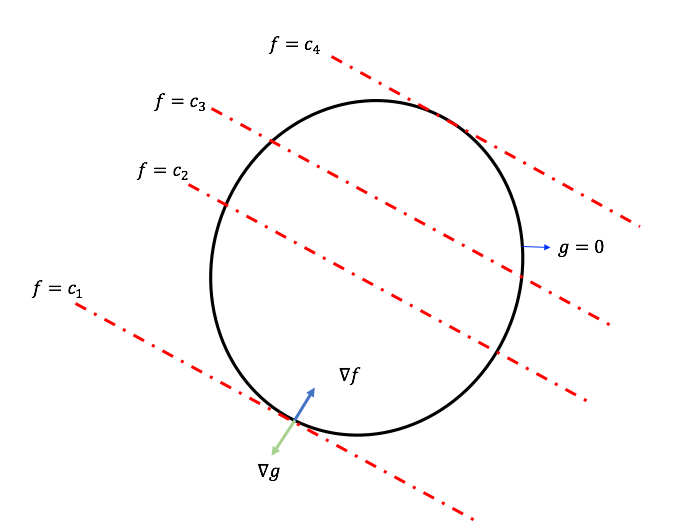
\includegraphics[width=10cm]{week13/F_13_1}
\caption{Illustration of Lagrange Multiplier Theorem}
\end{figure}
Here the circile denotes the set $\{(x,y,z)\mid g(x,y,z)=0\}$; the red line denotes the level set $\{(x,y,z)\mid f(x,y,z)=c_i\}$.

At the local minimum/maximum $(x,y,z)$, the cost gradient 
\[
\nabla f(x,y,z)=(1,-1,0)
\] is normal to the constraint surface, and is therefore, colinear with the constraint gradient
\[
\nabla h(x,y,z)=(2x,2y,2z).
\]
Suppose $\nabla f(x,y,z)-\lambda\nabla g(x,y,z)=0$, we obtain:
\begin{align*}
1-2\lambda x&=0\\
1-2\lambda y&=0\\
0-\lambda2z&=0
\end{align*}
This nonlinear system of equations has 4 unknowns and 3 equations, and therefore impossible to solve. Combining with the additional constraint equation $0=g(x,y,z)$, we are able to solve it:
\[
(x,y,z)=(\pm\frac{\sqrt{2}}{2},\mp\frac{\sqrt{2}}{2},0),\qquad
\lambda=\pm\sqrt{2}
\]
These two points are candidates for extreme points. Since the constraint set is compact, this optimization problem admits its global extreme points. Therefore, it is clear that $(\frac{\sqrt{2}}{2},-\frac{\sqrt{2}}{2},0)$ is the global maximum; and $(x,y,z)=(-\frac{\sqrt{2}}{2},\frac{\sqrt{2}}{2},0)$ is the global minimum
\end{example}

\begin{proof}\qquad\\
\begin{enumerate}
\item[Step 1: ]
Show that the tangent plane of the constraint set $\mathcal{S}:=\{\bm x:g(\bm x)=\bm c\}$ at $\bm x_0$ is given by:
\begin{equation}
T_{\bm x_0}(\mathcal{S})=\{\bm v\in\mathbb{R}^m\mid\inp{\nabla g(\bm x_0)}{\bm v}=0\}
\end{equation}
\item[Step 2:]
Show that $\nabla f(\bm x_0)\perp\bm v$, for $\forall\bm v\in T_{\bm x_0}(\mathcal{S})$: Fix $\bm v\in T_{\bm x_0}(\mathcal{S})$, then there exists a path $c(t)\in\mathcal{S}$ such that $c'(0)=\bm v$ and $c(0)=\bm x_0$.

Set $\phi(t)=f(c(t))$, the necessary condition for unconstraint optimization implies that
\[
0=\phi'(0)=\inp{\nabla f(c(t))}{c'(0)}|_{t=0}=\inp{\nabla f(\bm x_0)}{c'(0)}=\inp{\nabla f(\bm x_0)}{\bm v}.
\]
\end{enumerate}
\end{proof}
